% Created 2026-04-11 Sat 22:14
% Intended LaTeX compiler: pdflatex
\documentclass[11pt]{article}
\usepackage[utf8]{inputenc}
\usepackage[T1]{fontenc}
\usepackage{graphicx}
\usepackage{longtable}
\usepackage{wrapfig}
\usepackage{rotating}
\usepackage[normalem]{ulem}
\usepackage{amsmath}
\usepackage{amssymb}
\usepackage{capt-of}
\usepackage{hyperref}
\author{Danilo Unapucha,}
\date{2026-04-11}
\title{Taller de Configuracion de Entorno WSL}
\hypersetup{
 pdfauthor={Danilo Unapucha,},
 pdftitle={Taller de Configuracion de Entorno WSL},
 pdfkeywords={},
 pdfsubject={},
 pdfcreator={Emacs 27.1 (Org mode 9.7.5)}, 
 pdflang={Espanol}}
\begin{document}

\maketitle
\section{Actividades}
\label{sec:org0278664}
\subsection{Configuración de WSL con Ubuntu, \LaTeX{}, Python e Emacs}
\label{sec:org4166b30}

\begin{enumerate}
\item Verificación de entorno mamba/anaconda
\end{enumerate}
\begin{figure}[htbp]
\centering
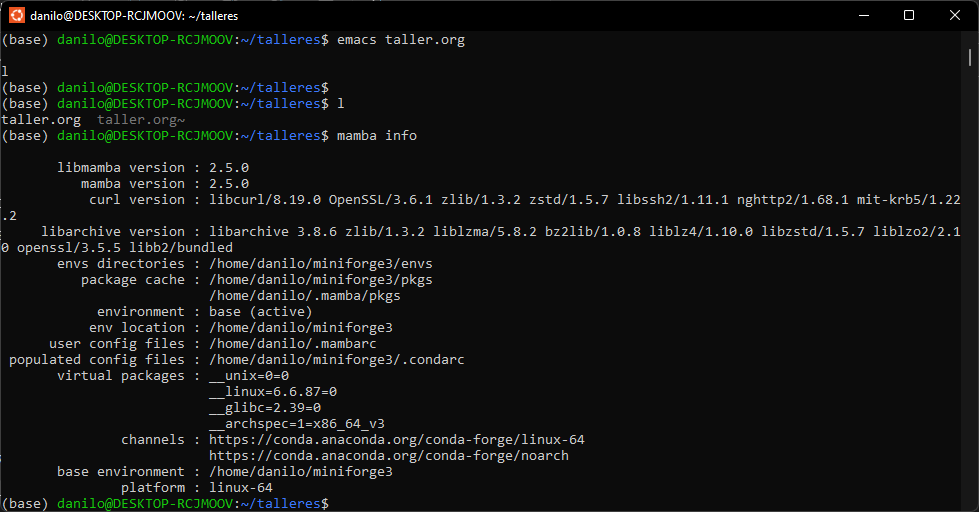
\includegraphics[width=.9\linewidth]{./images/mamba.png}
\caption{Evidencia de la configuración de Mamba Info en WSL}
\end{figure}

\begin{enumerate}
\item Verificación de Python
\end{enumerate}
\begin{figure}[htbp]
\centering
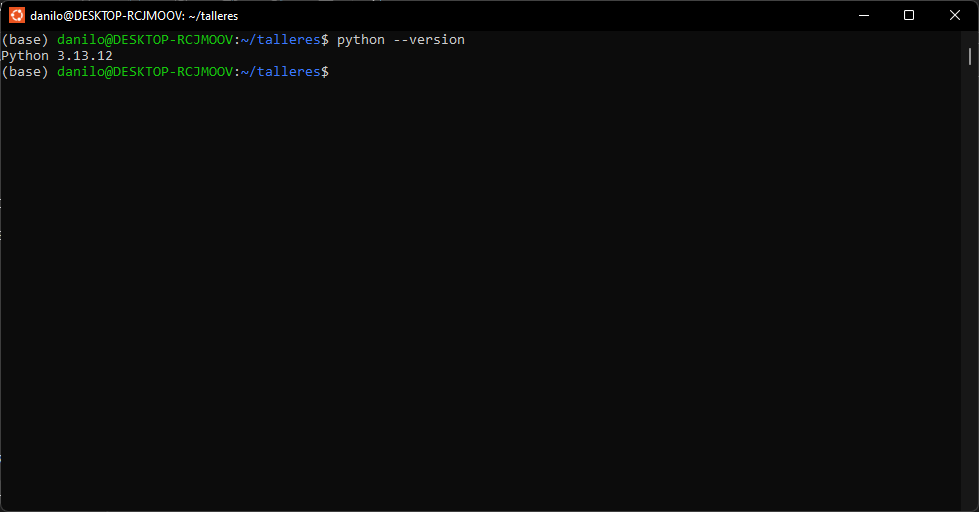
\includegraphics[width=.9\linewidth]{./images/python.png}
\caption{Versión de Python 3}
\end{figure}

\begin{enumerate}
\item Verificación de Emacs
\end{enumerate}
\begin{figure}[htbp]
\centering
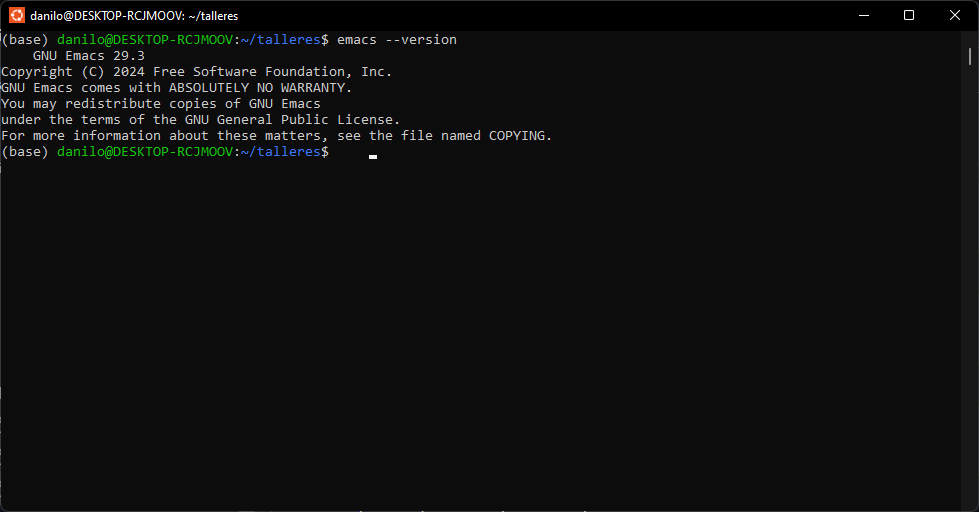
\includegraphics[width=.9\linewidth]{./images/emacs.png}
\caption{Versión de Emacs ejecutándose en modo ventana/terminal}
\end{figure}

\begin{enumerate}
\item Verificación de \LaTeX{}
\end{enumerate}
\begin{figure}[htbp]
\centering
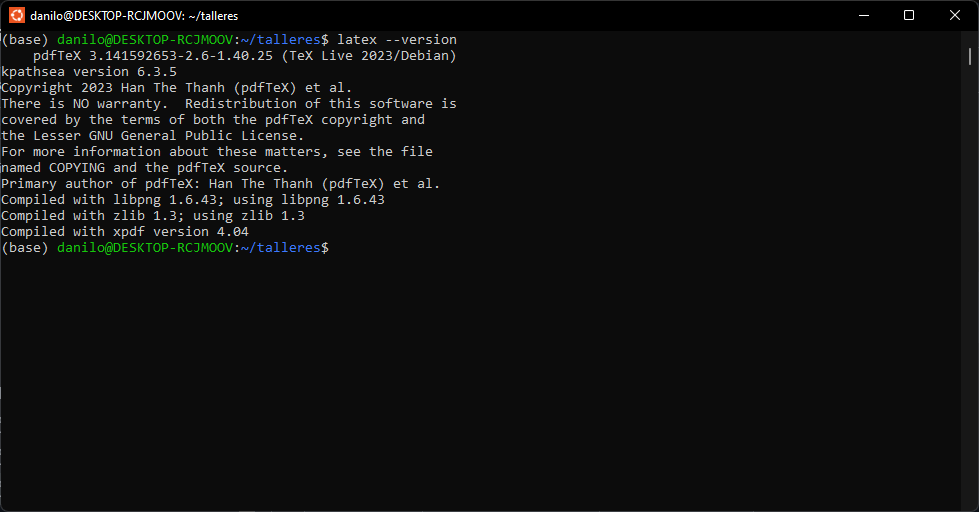
\includegraphics[width=.9\linewidth]{./images/latex.png}
\caption{Compilador \LaTeX{}}
\end{figure}
\subsection{Comandos emacs tutorial}
\label{sec:org5d7e27a}
Danilo Unapucha
\begin{center}
\begin{tabular}{llll}
Comando & Descripción & Comando & Descripción\\[0pt]
\hline
C-l & Me ayuda a ver de mejor manera el texto ya que me lo pone arriba o en la mitad o abajo & C-k & Ayuda mucho al poder elimar toda la linea en la que me encuetro\\[0pt]
M-k & Este elimina toda una oracion y ayuda bastante al eliminar todo un parrafo si no se esta conforme & C-g & Este es el mas importante ya que cierra el minibuffer o el comando para sacarnos de un apuro\\[0pt]
\end{tabular}
\end{center}
aqui va lo suyo michae sebas y otro
\subsection{Comandos Emacs Juego}
\label{sec:orgce39770}
Danilo Unapucha
\begin{center}
\begin{tabular}{rr}
Iteracion & Puntaje\\[0pt]
\hline
1 & 140\\[0pt]
2 & 140\\[0pt]
3 & 140\\[0pt]
\end{tabular}
\end{center}
\begin{enumerate}
\item Iteracion 1
\begin{center}
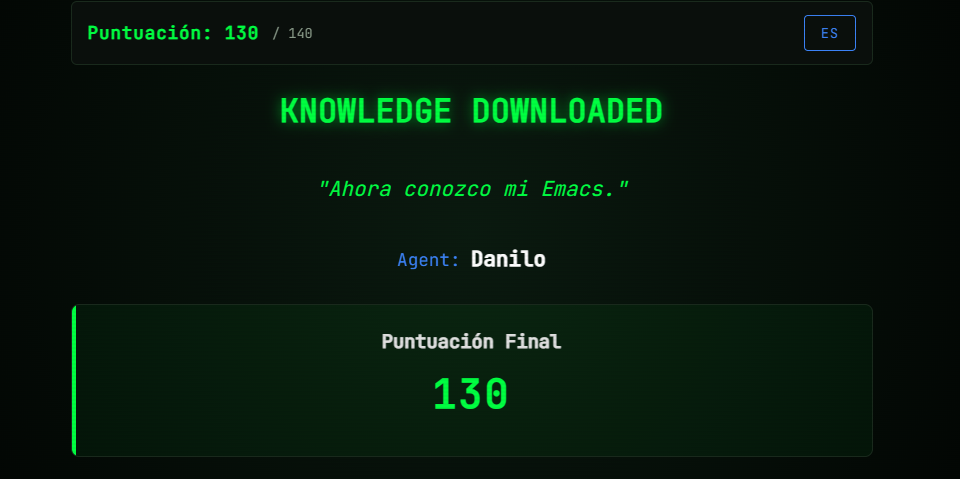
\includegraphics[width=.9\linewidth]{./images/juego1.png}
\end{center}
\item Iteracion 2
\begin{center}
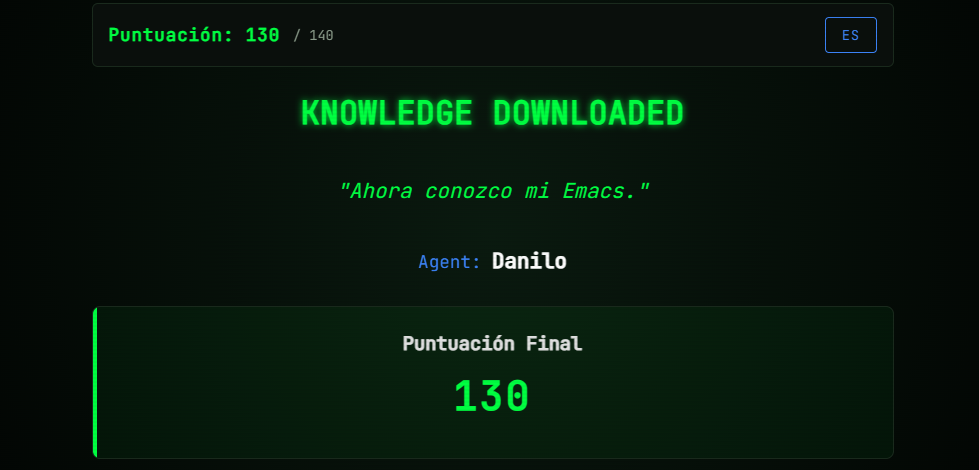
\includegraphics[width=.9\linewidth]{./images/juego2.png}
\end{center}
\item Iteracion 3
\begin{center}
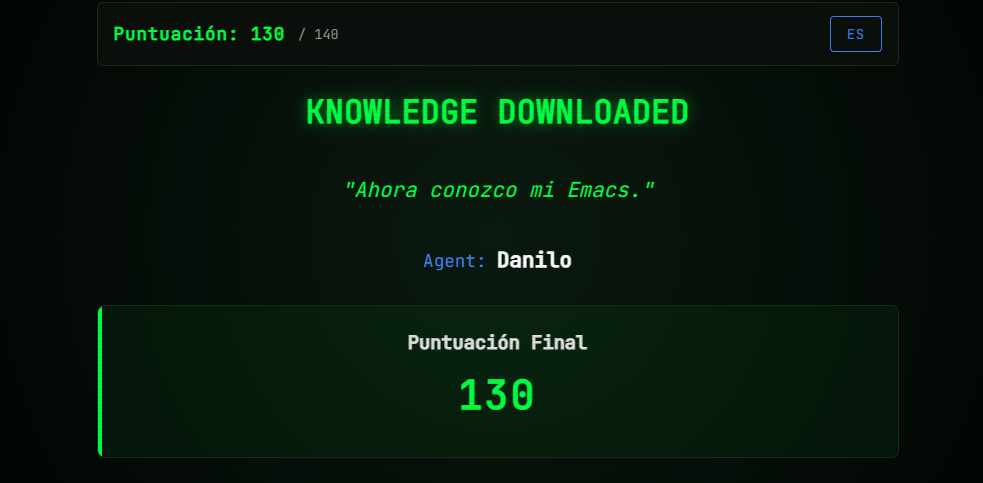
\includegraphics[width=.9\linewidth]{./images/juego3.png}
\end{center}
\end{enumerate}
lo suyo
\subsection{Usando Emacs para tener Ayuda sobre Emacs}
\label{sec:orge6ff53c}
\textbf{\textbf{Comandos Fáciles}}
\begin{enumerate}
\item \textbf{\textbf{Danilo Unapucha}} C-n. Move cursor vertically down ARG lines.
\item siguiente persona
\item 

\item 
\end{enumerate}
\textbf{\textbf{Comandos Dificiles}}
\begin{enumerate}
\item \textbf{\textbf{Danilo Unapucha}} C-v. Scroll text of selected window upward ARG lines; or near full screen if no ARG.
\item 

\item 

\item 
\end{enumerate}
\subsection{Equipo de Trabajo}
\label{sec:orgc28c036}
\begin{center}
\begin{tabular}{lll}
Nombre & email & Rol\\[0pt]
\hline
Danilo Unapucha & danilo.unapucha@epn.edu.ec & Colaborador\\[0pt]
 &  & \\[0pt]
 &  & \\[0pt]
 &  & \\[0pt]
\end{tabular}
\end{center}
\subsection{Verificación de Entregables}
\label{sec:org0bcb848}
\begin{itemize}
\item[{$\square$}] Verificación de configuración de entorno WSL y paquetes del curso.
\item[{$\square$}] Tutorial de Comandos Emacs realizado.
\item[{$\square$}] Captura de Imágenes y puntajes de Emacs Trainer App.
\item[{$\square$}] Usando Emacs para tener ayuda sobre Emacs
\item[{$\square$}] Verifique que estén los nombres de los integrantes del equipo e identificado el líder.
\item[{$\square$}] Revisión de ortografía con ispell en el buffer
\item[{$\square$}] Generación de Archivo PDF M-x org-latex-export-to-pdf
\end{itemize}
\end{document}
